\section{O Algoritmo CDI}\visiblelbl{sec:algoritmo}

A base do método é o uso do que chamamos de cilindros de confiança.
Esses cilindros são regiões ao redor do conjunto factível, definidas
por
\begin{equation}\visiblelbl{def:cilindro}
 \mathcal{C}(\rho) = \{z \in \Rn{n} : \norma{h(z)} \leq \rho\}.
\end{equation}
O método é dividido em passos normais e tangentes. Os passos
normais servem para aproximar os iterandos da região factível e
os passos tangentes tentam melhorar o progresso dual, segundo uma medida de
otimalidade.
A Figura \ref{fig:cilindro3d} esboça o processo.
\documentclass{standalone}
\usepackage[utf8]{inputenc}
\usepackage[T1]{fontenc}
\usepackage{pgfplots}
\pgfplotsset{compat=1.8}

\newcommand{\norma}[1]{\Vert #1 \Vert}

\begin{document}
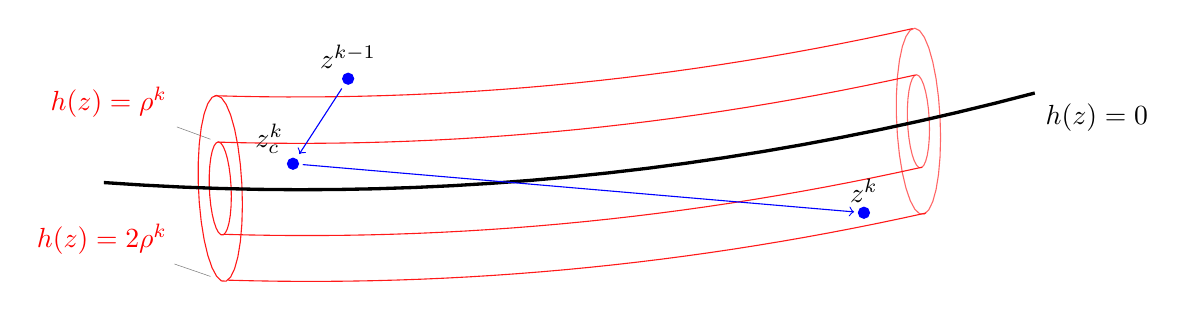
\begin{tikzpicture}
  \begin{axis}[view={70}{20}, xmin=-4.4, xmax=3.4, zmin=-1, ymax=-1.8, ymax=1.8,
      axis lines=none,
      xtick=\empty, ytick=\empty, ztick=\empty, x post scale=2.0,
      y post scale=2.5, z post scale=1.1, lightgray
    ]

    \addplot3 [domain=0:360, draw=red!90!white,
      samples=30, samples y=0]
        ({0.3*cos(x)}, {-1.2}, {0.1*1.2*1.2 + 0.3*sin(x)})
        node[pos=0.25, pin=160 : {\color{red}$\norma{h(z)}=\rho^k$}] {};
    \addplot3 [domain=0:360, draw=red!90!white,
      samples=30, samples y=0]
        ({0.6*cos(x)}, {-1.2}, {0.1*1.2*1.2 + 0.6*sin(x)})
        node[pos=0.75, pin=160 : {\color{red}$\norma{h(z)}=2\rho^k$}] {};
    \addplot3 [domain=0:360, draw=red!60!white,
      samples=30, samples y=0]
        ({0.3*cos(x)}, {1.2}, {0.1*1.2*1.2 + 0.3*sin(x)});
    \addplot3 [domain=0:360, draw=red!60!white,
      samples=30, samples y=0]
        ({0.6*cos(x)}, {1.2}, {0.1*1.2*1.2 + 0.6*sin(x)});

    \addplot3[domain=-1.6:1.6, samples y=0, very thick, draw=black]
      ({0}, {x}, {0.1*x^2})
      node [pos=1, below right] {\color{black} $h(z) = 0$};

    \foreach \t in {105,290} {
      \addplot3 [domain=-1.2:1.2,
        draw=red!90!white, samples=30, samples y=0]
        ({0.3*cos(\t)}, {x}, {0.1*x^2 + 0.3*sin(\t)});
       \addplot3 [domain=-1.2:1.2,
        draw=red!90!white, samples=30, samples y=0]
        ({0.6*cos(\t)}, {x}, {0.1*x^2 + 0.6*sin(\t)});
    }

    \addplot3+[solid, draw=blue, mark=*, only marks, mark options={fill=blue}] coordinates {
      (1.1,-0.9,1.0)  (0,-0.95,0.26) (0.1, 1.0, -0.4)
    }
      node [pos=0,above] {\color{black}$z^{k-1}$}
      node [pos=0.35,above left] {\color{black}$z_c^k$}
      node [pos=1,above] {\color{black}$z^k$};
      \node (x0) at (axis cs:1.1,-0.9,1.0) {};
      \node (xc) at (axis cs:0,-0.95,0.26) {};
      \node (x1) at (axis cs:0.1,1.0,-0.4) {};
      \draw[blue,->] (x0) -- (xc);
      \draw[blue,->] (xc) -- (x1);
  \end{axis}
\end{tikzpicture}
\end{document}

Utilizamos como medida de otimalidade a norma do gradiente projetado
aproximado na itera\c{c}\~ao $k$, denotado por $g_p^k$, e 
escolhemos raios dos cilindros de confiança proporcionais a essa medida, isto é,
$$ \rho^k = \bigo(\norma{g_p^k}). $$
Nossas itera\c{c}\~oes devem ser mantidas estritamente fact\'iveis em
rela\c{c}\~ao aos limitantes das vari\'aveis, isto \'e, devemos ter $s >
0$. 
Para garantir isso, dada a direção $d$ a partir de um ponto $z$, calculamos um
tamanho máximo de passo $\alpha$, tal que a nova itera\c{c}\~ao satisfaça
\begin{equation}\visiblelbl{eq:slim}
s + \alpha d_s \geq \epsmu s
\end{equation}
para algum $\epsmu > 0$ pequeno dado, onde $d_s$ é
a componente do vetor $d$ correspondente às variáveis $s$. 
Um esboço do método está descrito no Algoritmo \ref{alg:outline}.
\begin{algorithm}[H]
\caption{Método CDI}
\visiblelbl{alg:outline}
\begin{algorithmic}[1]
\State Parâmetros: $\varepsilon_g > 0$, $\varepsilon_h > 0$, $\varepsilon_a >
0$, $\epsmu \in (0,1)$ e $\nu \in [10^{-4},1]$.
\State Valores Iniciais: $z^0$, $\rho^0 > 0$, $\mu^0$, $k = 1$, $\rhomax^0$.
\State \visiblelbl{alg.step:comeco}Faça a {\bf Etapa Normal}, encontrando $z_c^k$,
  $\lk{k}$, $\rho^k$, $\mu^k$ e $g_p^k = g(z_c^k,\mu^k) + A(z_c^k)^T\lk{k}$
  tais que \visiblelbl{alg:normal-call}
    $$ \norma{h(z_c^k)} \leq \rho^k \leq \nu \frac{\norma{g_p^k}\rhomax^{k-1}}
    {\norma {g(\zc{k},\mu^k)} + 1}, \qquad \mbox{e} \qquad s_c^k \geq \epsmu
    s^{k-1} $$
  \If{ $\norma{h(z_c^k)} < \varepsilon_h$, $\norma{g_p^k} < \varepsilon_g$ e
    $\modulo{(s_c^k)^T\lk{k}} < \varepsilon_a$ }
  \State PARE com $z^* = z_c^k$.
\EndIf
\State Faça a {\bf atualização de $\rhomax^k$}.
\State Faça a {\bf Etapa Tangente}, encontrando $z_k$ com decréscimo suficiente
para a função Lagrangeana e tal que \visiblelbl{alg:tangente-call}
$$ \norma{h(z^k)} \leq 2\rho^k \qquad \mbox{e} \qquad s^k \geq \epsmu s_c^k. $$
\State Incremente $k$ e volte para o passo \ref{alg.step:comeco}.
\end{algorithmic}
\end{algorithm}
A etapa normal do método é composta do cálculo do passo normal e da atualização
dos multiplicadores e do gradiente projetado. 
Os requerimentos sobre o formato desse passo s\~ao poucos, como veremos
posteriormente. Escolhemos encontrar um passo normal com uma sequ\^encia de
itera\c{c}\~oes de algum m\'etodo para resolver o problema 
\begin{equation}\visiblelbl{prob:normal}
\begin{array}{rl}
  \min &\dfrac{1}{2}\norma{h(z)}^2 \\
  \mbox{suj. a} & s \geq 0.
\end{array}
\end{equation}
Nossa estrat\'egia consiste em encontrar um $z_c$ dentro do cilindro de raio 
$\rho$, atualizar o raio, e verificar se $z_c$ permanece dentro do cilindro.
Caso n\~ao permane\c{c}a, repetimos o processo. Cada aplica\c{c}\~ao do m\'etodo
inicia no ponto $z_c$ anterior, sendo que o primeiro $z_c$ da iteração $k$ é
escolhido como $z_c = z^{k-1}$. 
Cada passo que leva a um ponto dentro do cilindro é dito um {\bf passo normal
interno}.
Definimos os subproblemas normais como
\begin{equation}\visiblelbl{prob:normal_direction}
\begin{array}{rl}
  \min & \dfrac{1}{2}\norma{h(z_c+d)}^2 \\
 \mbox{suj. a} & \ell_N \leq d \leq u_N,
\end{array}
\end{equation}
onde 
\begin{equation}\visiblelbl{eq:normal_bounds_definition}
  \ell_N = \vetor{-\Delta_Ne_n}{-\min\{\Delta_Ne_m,(1-\epsmu)s^{k-1}\}}
  \qquad\mbox{e}\qquad u_N = \Delta_Ne_{n+m},
\end{equation}
com $e_n, e_m$ e $e_{n+m}$ são vetores com todas as componentes iguais a $1$, de
tamanho $n$, $m$ e $n+m$, respectivamente.
O Algoritmo \ref{alg:etapa.normal} mostra o esboço da etapa normal.
\begin{algorithm}[H]
\caption{Etapa Normal}
\visiblelbl{alg:etapa.normal}
\begin{algorithmic}[1]
\State Parâmetros: $\alpha_\rho > 0$ e $\alpha_h > 0$.
\State Valores Iniciais: $z_c = z^{k-1}$.
\State Calcule $\lambda$, $g_p = g(z_c,\mu) + A(z_c)^T\lambda$, $\rho$ e
  $\mu$.
\While{ $\norma{h(z_c)} > \rho$ }
  \State Encontre $z_c$ tal que $\norma{h(z_c)} \leq \rho$ e $s_c \geq \epsmu
    s^{k-1}$ pelo {\bf passo normal interno}.
  \State Calcule $\lambda$, $g_p = g(z_c,\mu) + A(z_c)^T\lambda$, $\rho$ e
    $\mu$.
\EndWhile
\State Defina $\lambda^k = \lambda$, $g_p^k = g_p$ e $\rho^k = \rho$.
\State Defina $\mu^k = \min\bigg\{ \mu^{k-1}, \alpha_\rho\rho,
  \alpha_\rho\rho^2, \dfrac{(s_c^k)^T\max\{0,-\lambda_I^k\}}{m_I},
  \alpha_hh(z^k)\bigg\}.$
  \visiblelbl{alg:mudef}
\end{algorithmic}
\end{algorithm}
No algoritmo, calculamos $\lk{k}$ de maneira que fique pr\'oximo a
$\lambda_{LS}(\zc{k} ,\mu^k)$, mas garantimos que o sinal dos multiplicadores
associados \`as desigualdades estejam corretos quando $\mu$ tende a $0$. 
Esse c\'alculo \'e feito como
\begin{equation}\visiblelbl{def:lambda}
  \lambda_i^k = \left\{
    \begin{array}{ll}
      \lambda_{LS_i}(\zc{k},\mu^k), & \mbox{se } i \in E \\ 
      \min\{\lambda_{LS_i}(\zc{k},\mu^k), \alpha(\mu_k)^r\}, & \mbox{se } i \in I \\ 
    \end{array}
  \right.
\end{equation}
onde $\alpha > 0$ e $r > 0$ s\~ao escolhidos adequadamente.
Com esse multiplicador, definimos o gradiente projetado aproximado
$\gpk{k}$ como 
\begin{equation} \visiblelbl{def:gpk}
\gpk{k} = g(\zc{k},\mu^k) + A(\zc{k})^T\lk{k}
= \vetor{ \nabla_x\mathcal{L}(x^k_c, \lk{k}) }
{-\mu^ke - S_c^{k+1}\lk{k}_I},
\end{equation}
de modo que $\gpk{k}$ ficar\'a pr\'oximo
de $g_p(\zc{k},\mu^k).$

A etapa tangente é responsável por diminuir a infactibilidade dual, calculando
um passo tangente que forneça decréscimo suficiente.
O passo é obtido utilizando uma aproximação quadrática para o Lagrangeano e
regiões de confiança, com a direção escalada pela matriz $\Lambda(z_c^k)$. 
Lembramos aqui que, para evitar o mal condicionamento, utilizamos uma aproximação
quadrática de $L(z_c^k + \Lambda(z_c^k)\delta, \lk{k}, \mu^k)$.
Além do decréscimo, o ponto não pode sair do cilindro
$\mathcal{C}(2\rho^k)$.
O passo tangente $\delta_t$ \'e obtido atrav\'es da solu\c{c}\~ao aproximada para o
problema
\begin{equation}\visiblelbl{prob:tangente}
  \begin{array}{rcl}
  \displaystyle\min_{\delta} & & q_k(\delta) = \dfrac{1}{2}\delta^TB^k\delta +
  \delta^Tg_p^k \\
 \mbox{suj. a} & & A(\zc{k})\delta = 0 \\
               & & \ell_T \leq \Lambda(z_c^k)\delta \leq u_T,
  \end{array}
\end{equation}
onde $B^k$ \'e uma aproxima\c{c}\~ao para $W(\zc{k},\lk{k},\mu^k)$, e
os limitantes $\ell_T$ e $u_T$ têm o mesmo formato daqueles definidos
em \eqref{eq:normal_bounds_definition},
mas com uma regi\~ao de confian\c{c}a de raio $\Delta_T$, e $s_c^k$ no lugar de
$s^{k-1}$.
Pedimos que o passo encontrado
seja ao menos melhor que um passo de Cauchy. Então, utilizamos uma implementação
que começa com o passo de Cauchy e tenta melhorar o valor da quadrática, até ser
forçado a parar pelos limitantes, ou ao obter um minimizador da quadrática.
Após o passo tangente, ainda podemos fazer uma correção de segunda ordem, 
conforme sugerido em \cite{bib:book-conn-trust}. Mostraremos como, e quando, é
feita essa correção na Subseção \ref{subsec:soc}.
O ponto obtido pelo passo tangente e pela correção de segunda ordem é o próximo
iterando $z^k$.
O algoritmo \ref{alg:etapa.tangente} mostra um esboço da etapa tangente.
\begin{algorithm}[H]
\caption{Etapa Tangente}
\visiblelbl{alg:etapa.tangente}
\begin{algorithmic}[1]
\State Parâmetros: $\eta_1 \in (0,\meio]$, $\eta_2 > \eta_1$, $\alpha_R \in
(0,\frac{3}{4}]$, $\alpha_I > 1$.
\State Valores Iniciais: $\Delta_T$, $r = 0$ e $z^+ = z_c^k$.
\While{ $\norma{h(z^+)} > 2\rho^k$ ou $r < \eta_1$ }
  \visiblelbl{alg:tangente-condicoes}
  \State Construa $\ell_T$ e $u_T$ usando $\Delta_T$.
  \State Calcule o Passo de Cauchy $\delta_{CP} = -\alpha_{CP}g_p^k$, onde
  $\alpha_{CP}$ é solução de 
    \visiblelbl{alg:cauchy-point}
  \begin{eqnarray*}
    \min_{\alpha > 0} & & q(-\alpha g_p^k) \\
    \mbox{suj. a}  & & \ell_T \leq -\alpha \Lambda(z_c^k) g_p^k \leq u_T.
  \end{eqnarray*}
  \State Calcule um {\bf passo tangente interno} $\delta_t$ tal que
    \visiblelbl{alg:delta-t}
    \begin{eqnarray*}
      q(\delta_t) & \leq & q(\delta_{CP}), \\
      A(z_c^k)\delta_t & = & 0, \\
      \ell_T & \leq & \Lambda(z_c^k)\delta_t \quad \leq \quad u_T.
    \end{eqnarray*}
  \State Se necessário, calcule uma correção de segunda ordem $\dsoc$.
  \State $\dplus = \Lambda(z_c^k) (\delta_t + \dsoc)$.
  \State $z^+ = z_c^k + \dplus$
    \visiblelbl{alg:tangente-plus}
  \State $\Delta L_T^k = L(z^+,\lk{k},\mu^k) - L(z_c^k,\lk{k},\mu^k)$
  \State $r = \dfrac{ \Delta L_T^k }{ q(\delta_t) }$
  \If{ $\norma{h(z^+)} > 2\rho^k$ OU $r < \eta_1$ }
    \State $\Delta_T = \alpha_R\Delta_T$
  \ElsIf{ $r > \eta_2$ }
    \State $\Delta_T = \alpha_I\Delta_T$
  \EndIf
\EndWhile
\State Defina $z^k = z^+$
\end{algorithmic}
\end{algorithm}

Al\'em da norma do gradiente projetado na itera\c{c}\~ao $k$, tamb\'em usamos
a varia\c{c}\~ao do Lagrangeano para controlar o tamanho do raio do cilindro.
Para explicitarmos a contribuição dos passos normal e tangente, dividimos a
variação do Lagrangeano calculado logo após o passo normal em
\begin{equation}\visiblelbl{DLC}
  \Delta \Lc{k} = \Lc{k} - \Lc{k-1} = \DLH{k-1} + \DLV{k},
\end{equation}
onde 
\begin{eqnarray}
  \Lc{k} & = & L(\zc{k},\lk{k},\mu^k), \nonumber \\
 \DLH{k} & = & L(z^k,\lk{k},\mu^k) - L(\zc{k},\lk{k},\mu^k) \visiblelbl{DLH}, \\
 \DLV{k} & = & L(\zc{k},\lk{k}, \mu^k) - L(z^{k-1},\lk{k-1},\mu^{k-1}).
  \visiblelbl{def:DLN}
\end{eqnarray}
A maneira que a atualização de $\rhomax$ é feita está descrita no Algoritmo
\ref{alg:update.rhomax}.
\begin{algorithm}[H]
\caption{Atualização de $\rhomax$}
\visiblelbl{alg:update.rhomax}
\begin{algorithmic}[1]
\State Valores Iniciais: $\Lref$ definido em iterações anteriores.
  Inicialmente $\Lref = \infty$.
\State $\Delta L_N^k = L(z_c^k,\lk{k},\mu^k) - L(z^{k-1},\lk{k-1},\mu^{k-1})$
\If{ $\Delta L_N^k \geq \meio[\Lref - L(z^{k-1},\lk{k-1},\mu^{k-1})]$ }
\visiblelbl{alg:update-rhomax-start}
  \State $\rhomax^k = \rhomax^{k-1}/2$
\Else
  \State $\rhomax^k = \rhomax^{k-1}$
\EndIf
\visiblelbl{alg:update-rhomax-end}
\If{ $\Delta L_N^k > -\meio \Delta L_T^{k-1}$ }
  \visiblelbl{alg:condicao-dlv}
  \State $\Lref = L(\zc{k},\lk{k},\mu^k)$
\EndIf
\end{algorithmic}
\end{algorithm}

\ifdraft
\else
Para deixar mais claro o funcionamento do método, vamos aplicar o algoritmo à
dois exemplos. O primeiro é o problema
\begin{eqnarray}
  \min & f(x) = \meio(x_1^2 + x_2^2) \nonumber \\
  \mbox{s.t} & x_2 = x_1^2 + 1, \nonumber
\end{eqnarray}
cuja solução é o ponto $(1,0)$.

\newcommand{\addexum}[1]{
  \includegraphics[scale=1.0]{ex1_plots/ex1_img#1.pdf}
}

\begin{center}
  \addexum{1}
\end{center}

\begin{center}
  \begin{minipage}{0.9\textwidth}
  Começamos pelo ponto $x_0 = \vetor{2}{3}$, denotado pelo círculo sólido na imagem.
  A curva sólida representa a região factível, as curvas tracejadas 
  denotam o cilindro menor e as curvas pontilhadas denotam o cilindro
  maior. As circunferências concêntricas denotam as curvas de nível da função objetivo, cujo
  menor valor ocorre na origem.
\end{minipage}
\end{center}

\begin{center}
  \addexum{2}
\end{center}

\begin{center}
  \begin{minipage}{0.9\textwidth}
  Iniciamos notando que o ponto não está dentro do cilindro menor. Então
  fazemos um passo normal. O ponto obtido, denotado $x_c$, é a tentativa de
  iterando. Como o ponto já está dentro do cilindro
  menor, o passo é interrompido.
\end{minipage}
\end{center}

\begin{center}
  \addexum{3}
\end{center}

\begin{center}
  \begin{minipage}{0.9\textwidth}
  Agora, atualizamos o raio dos cilindros. Como o $x_c$ obtido continuou
  dentro do cilindro menor após o raio deste ter sido atualizado, definimos
  $x_c^0$ como este iterando normal.
\end{minipage}
\end{center}

\begin{center}
  \addexum{4}
\end{center}

\begin{center}
  \begin{minipage}{0.9\textwidth}
  A partir deste ponto, tentamos realizar um passo tangente. O raio da região de
  confiança, não ilustrado na imagem, é grande o suficiente para permitir que o
  passo seja tomado completamente. O passo aqui é o minimizador da aproximação
  quadrática do Lagrangeano. $x^+$. Nesse caso, como esse ponto está fora do
  cilindro maior, rejeitamos o passo e reduzimos a
  região de confiança.
\end{minipage}
\end{center}

\begin{center}
  \addexum{5}
\end{center}

\begin{center}
  \begin{minipage}{0.9\textwidth}
  Calculamos um novo passo tangente, desta vez limitado pela região de
  confiança, indicada pelo segmento tracejado. Note que, na verdade, este
  segmento faz parte da caixa que é a região de confiança.
  O iterando $x^+$ obtido está dentro do cilindro maior e fornece decréscimo
  suficiente, sendo portanto aceito como o próximo iterando.
\end{minipage}
\end{center}

\begin{center}
  \addexum{6}
\end{center}

\begin{center}
  \begin{minipage}{0.9\textwidth}
  $x^1$ obtido pelo passo tangente.
\end{minipage}
\end{center}

\newpage
Para verificar a aplicação do método no caso com inequações, vamos apresentar
outro exemplo. Note, no entanto, que um problema de duas variáveis e uma
inequação precisaria ser analisado em 3 dimensões. Decidimos, para facilitar a
visualização, mostrar apenas as variáveis originais do problema, e utilizar a
definição da variável de folga para mostrar a restrição deslocada.
Pelo mesmo motivo, vamos mostrar apenas uma parte dos cilindros de confiança.

O problema que consideramos é
\begin{eqnarray}
  \min & f(x) = \meio[x_1^2 + (x_2+1)^2] \nonumber \\
  \mbox{suj. a} & x_2 \geq x_1^2, \nonumber \\
               & x_1 + x_2 = 1, \nonumber
\end{eqnarray}
cuja solução é o ponto $(\frac{-1+\sqrt{5}}{2},\frac{3-\sqrt{5}}{2}) \approx
(0.618,0.382)$.
Ao adicionarmos a variável de folga $s$, obtemos o problema
\begin{eqnarray}
  \min & f(x) = \meio[x_1^2 + (x_2+1)^2] \nonumber \\
  \mbox{suj. a} & x_2 - x_1^2 = s, \nonumber \\
               & x_1 + x_2 = 1, \nonumber \\
               & s \geq 0. \nonumber
\end{eqnarray}
Na solução, o valor de $s$ é $0$.

Os cilindros de confiança para esse problema serão os conjuntos da forma
$$ \mathcal{C}(\rho) = \{(x,s) \in \mathbb{R}^3: (x_2 - x_1^2 - s)^2 +
  (x_1+x_2-1)^2 \leq \rho^2\}. $$
Para mostrar alguma informação dessa região no plano original do problema,
decidimos tomar o caso com $s$ fixo. Dessa maneira, podemos ter alguma
informação do cilindro para as variáveis $x$. Note que essa visualização do
cilindro pode mudar de uma iteração para outra mesmo que o raio do cilindro
permaneça o mesmo.

\newcommand{\addexdois}[1]{
  \includegraphics[scale=1.0]{ex2_plots/ex2_img#1.pdf}
}

\begin{center}
  \addexdois{1}

  $s^0 = 0.01$
\end{center}

\begin{center}
  \begin{minipage}{0.9\textwidth}
    Começamos este exemplo pelo ponto $x^0 = (1,-1)$, e $s^0 = 0.01$, um valor
    pequeno e positivo.
    No gráfico, a reta corresponde à segunda equação; a região hachurada
    correspondente ao conjunto factível da desigualdade; e a parábola sólida
    corresponde à equação $x_2 - x_1^2 = s^0$.
    A curva tracejada denota o corte do cilindro pequeno em $s = s^0$, e a
    pontilhada o corte do cilindro grande pelo mesmo plano.
\end{minipage}
\end{center}

\begin{center}
  \addexdois{2}

  $s_c^0 = 0.01$
\end{center}

\begin{center}
  \begin{minipage}{0.9\textwidth}
    O ponto inicial já está dentro do cilindro pequeno, então o ponto é aceito
    sem necessidade de calcular nenhum passo normal.
  \end{minipage}
\end{center}

\begin{center}
  \addexdois{3}

  $s^+ = 14.15$
\end{center}

\begin{center}
  \begin{minipage}{0.9\textwidth}
    Tentamos agora fazer um passo tangente. O ponto encontrado fica fora do cilindro
    maior e não obtém decréscimo suficiente. Note que o cilindro não é
    visualizado, pois o corte é feito com o valor de $s$ encontrado resulta no
    conjunto vazio. Note que a parábola sólida também não é visualizada por
    causa do valor de $s$.
  \end{minipage}
\end{center}

\begin{center}
  \addexdois{4}

  $s^+ = 3.54$
\end{center}

\begin{center}
  \begin{minipage}{0.9\textwidth}
  O segundo passo tangente obtém decréscimo suficiente e está dentro do cilindro
  maior, que agora pode ser visualizado. Note que a parábola sólida também já
  pode ser visualizada.
\end{minipage}
\end{center}

\begin{center}
  \addexdois{5}

  $s^1 = 3.54$
\end{center}

\begin{center}
  \begin{minipage}{0.9\textwidth}
    O ponto é aceito como iteração tangente.
  \end{minipage}
\end{center}

\begin{center}
  \addexdois{6}

  $s_c = 1.29$
\end{center}

\begin{center}
  \begin{minipage}{0.9\textwidth}
    Atualizamos o raio do cilindro e fazemos um passo normal, levando o ponto
    para dentro do cilindro menor.
  \end{minipage}
\end{center}

\begin{center}
  \addexdois{7}

  $s_c^2 = 1.29$
\end{center}

\begin{center}
  \begin{minipage}{0.9\textwidth}
    Atualizamos novamente o raio do cilindro e o ponto encontrado permance dentro do
    cilindro menor. Portanto encerramos o passo normal.
  \end{minipage}
\end{center}

\begin{center}
  \addexdois{8}

  $s^+ = 1.03$
\end{center}

\begin{center}
  \begin{minipage}{0.9\textwidth}
    Fazemos um passo tangente, que fica dentro do cilindro e também tem
    decréscimo suficiente.
\end{minipage}
\end{center}

\begin{center}
  \addexdois{9}

  $s^2 = 1.03$
\end{center}

\begin{center}
  \begin{minipage}{0.9\textwidth}
    Aceitamos o ponto.
  \end{minipage}
\end{center}

\begin{center}
  \addexdois{10}

  $s_c = 0.67$
\end{center}

\begin{center}
  \begin{minipage}{0.9\textwidth}
    Fazemos um passo normal.
  \end{minipage}
\end{center}

\begin{center}
  \addexdois{11}

  $s_c^3 = 0.67$
\end{center}

\begin{center}
  \begin{minipage}{0.9\textwidth}
    Aceitamos a iteração normal.
  \end{minipage}
\end{center}

\begin{center}
  \addexdois{12}

  $s^+ = 0.16$
\end{center}

\begin{center}
  \begin{minipage}{0.9\textwidth}
    Fazemos um passo tangente.
  \end{minipage}
\end{center}

\begin{center}
  \addexdois{13}

  $s^3 = 0.16$
\end{center}

\begin{center}
  \begin{minipage}{0.9\textwidth}
    Aceitamos a iteração tangente.
  \end{minipage}
\end{center}

\begin{center}
  \addexdois{14}

  $s_c = 0.06$
\end{center}

\begin{center}
  \begin{minipage}{0.9\textwidth}
    Fazemos um passo normal.
  \end{minipage}
\end{center}

\begin{center}
  \addexdois{15}

  $s_c^4 = 0.06$
\end{center}

\begin{center}
  \begin{minipage}{0.9\textwidth}
    Aceitamos a iteração normal. O algoritmo oscila mais algumas iterações ao
    redor da solução até chegar à precisão necessária para declarar
    convergência.
  \end{minipage}
\end{center}


\fi

%A Figura \ref{flux:outline} mostra um fluxograma do método. Por sua vez, as
%figuras \ref{flux:normal} e \ref{flux:tangent} detalham o passo normal e o 
%passo tangente, respectivamente.
%\begin{figure}[H]
%  \centering
%  \begin{tikzpicture}
%    \node[block] (normal) {Encontre $z_c^k$ do {\bf Passo Normal}};
%    \node[decision,below of=normal,node distance=6em] (opt) {O critério de
%      parada é satisfeito?};
%    \node[block,below of=opt,node distance=7em,text width=9em] (end) {FIM.
%    Retorne sucesso com $x^* = x_c^k$.};
%    \node[block,right of=opt,node distance=17em] (tangent) {Encontre $z^k$
%      através do {\bf Passo Tangente}};
%    \node[block,above of=tangent,node distance=6em,text width=7em] (kpp) {$k = k + 1$};
%
%    \algstart{normal}
%    \path[line] (normal) -- (opt);
%    \path[line] (opt) --node[right]{SIM} (end);
%    \path[line] (opt) --node[above]{NÃO} (tangent);
%    \path[line] (tangent) -- (kpp);
%    \path[line] (kpp) -- (normal);
%  \end{tikzpicture}
%  \caption{Esboço do Método}
%  \label{flux:outline}
%\end{figure}
%\begin{figure}[H]
%  \centering
%  \begin{tikzpicture}
%    \node[block] (update) {Atualize $\lambda$, $g_p$};
%    \node[block,below of=update,node distance=5em] (updaterho) {Atualize $\rho =
%      \bigo(\norma{g_p})$};
%    \node[decision,below of=updaterho,node distance=6em] (feasible)
%      {$z_c\in\mathcal{C}(\rho)$?};
%    \node[block,below of=feasible,node distance=7em] (find) {Encontre
%      $z_c\in\mathcal{C}(\rho)$ a partir de \eqref{prob:normal_direction}};
%    \node[block,right of=feasible,node distance=16em] (end) {FIM do {\bf Passo Normal}};
%
%    \algstart[Comece com $z_c = z^{k-1}$]{update}
%    \path[line] (update) -- (updaterho);
%    \path[line] (updaterho) -- (feasible);
%    \path[line] (feasible) --node[right]{NÃO} (find);
%    \path[line] (feasible) --node[above]{SIM} (end);
%    \path[line] (find) -| (-4,0) |- (update);
%  \end{tikzpicture}
%  \caption{Esboço do Passo Normal}
%  \label{flux:normal}
%\end{figure}
%\begin{figure}[H]
%  \centering
%  \begin{tikzpicture}
%    \node[block] (delta) {Encontre $\delta_t$ a partir de \eqref{prob:tangente}};
%    \node[decision,below of=delta,node distance=8.5em] (feasible) {$z_c^k + \delta_t\in
%      \mathcal{C}(2\rho)$ e fornece decréscimo suficiente?};
%    \node[block,below of=feasible,node distance=8.5em, text width=6cm] (soc) {Se necessário,
%      calcule uma correção de segunda ordem $\dsoc$. Caso contrário, $\dsoc = 0$};
%    \node[block,below of=soc,node distance=5.5em, text width=6cm] (accept) {$z^k =
%    z_c^k+\Lambda(z_c^k)(\delta_t+\dsoc)$ e fim do {\bf Passo Tangente}};
%    \node[block,left of=feasible,node distance=16em,text width=6em] (reduce) {Reduza $\Delta_T$};
%    \algstart{delta};
%
%    \path[line] (delta) -- (feasible);
%    \path[line] (feasible) --node[right] {SIM} (soc);
%    \path[line] (feasible) --node[above] {NÃO} (reduce);
%    \path[line] (soc) -- (accept);
%    \path[line] (reduce) |- (delta);
%  \end{tikzpicture}
%  \caption{Esboço do Passo Tangente}
%  \label{flux:tangent}
%\end{figure}
%
%\subsection{O Pseudo-Código}
%
%No Algoritmo \ref{alg:outline} apresentamos o método com mais detalhes.
%Alguns detalhes de implementação serão mostrados no Capítulo
%\ref{chap:implementacao}.
%\begin{algorithm}[H]
%\caption{Método CDI}
%\visiblelbl{alg:outline}
%\begin{algorithmic}[1]
%\State Parâmetros: 
%$\eta_1\in(0,\meio], 
%\eta_2 > \eta_1$,
%$\varepsilon_g$, $\varepsilon_h$, $\varepsilon_a$,
%$\varepsilon_{\mu} > 0$, 
%$\alpha_R \in (0,\frac{3}{4}],
%\alpha_I > 1$,
%$\nu \in [10^{-4}, 1]$.
%\State Valores Iniciais: $z^0$, 
%$\rho^0$, $\rhomax^0$, 
%$\mu^0 > 1$, $\Lref = \infty$,
%$k = 0$
%\State Faça $g_p^0 = g(z^0,\mu^0) + A(z^0)^T\lambda^0$
%\While{ $\norma{g_p^k} > \varepsilon_g$ ou $\norma{h(z^k)} > \varepsilon_h$ ou
%$(s^k)^T\lambda_I^k > \varepsilon_{a}$ }
%  \State $k=k+1$
%  \State $z_c = z^{k-1}$, $\rho = \rho^{k-1}$, $\mu = \mu^{k-1}$
%  \While{ $\norma{h(z_c)} > \rho$ } \Comment{Passo Normal}
%    \State Encontre um ponto $z_c \in \mathcal{C}(\rho)$ tal que
%    $s_c \geq \epsmu s^{k-1}$. Se não for possível, {\bf interrompa} o algoritmo
%      com falha.
%    \State Calcule $\lambda$ e $g_p$
%    \State Atualize $\rho = \nu \norma{g_p} \rhomax/(\norma{g}+1)$
%    \visiblelbl{alg:update-rho}
%  \EndWhile
%  \State Faça $\lambda^k= \lambda$, $g_p^k= g_p$, $\rho^k = \rho$, 
%  \State Faça $\mu^k = \min\bigg\{ \mu^{k-1}, \alpha_{\rho}\rho,
%    \alpha_{\rho}\rho^2, \dfrac{(s_c^k)^T\max\{0,-\lambda^k_I\}}{m_I}, 
%    \alpha_h h(z^k)\bigg\}$.\visiblelbl{alg:mudef}
%  
%  \State $\Delta L_N^k = L(\zc{k}, \lambda^k, \mu^k) -
%    L(z^{k-1}, \lambda^{k-1}, \mu^{k-1})$ 
%    \Comment{Atualização do $\rhomax$}
%  \If{$\Delta L_N^k \geq \meio[\Lref - L(z^{k-1}, \lambda^{k-1}, \mu^{k-1})]$}
%\visiblelbl{alg:condicao-lref}
%    \State $\rhomax^k = \rhomax^{k-1}/2$  
%  \Else
%    \State $\rhomax^k = \rhomax^{k-1}$  
%  \EndIf
%  \If{ $\Delta L_N^k > -\meio\Delta L_T^{k-1}$ } \visiblelbl{alg:condicao-dlv}
%    \State $\Lref = L(\zc{k}, \lambda^k, \mu^k)$
%  \EndIf
%  \State Defina $r = 0$ e $\zp = z_c^k$
%  \Comment{Passo Tangente}
%  \While{ $\norma{h(\zp)} > 2\rho^k$ ou $r < \eta_1$ } \visiblelbl{alg:tangente-condicoes}
%    \State Calcule o Passo de Cauchy $\delta_{CP} = -\alpha g_p^k$, em que
%    $\alpha$ é a solução de
%    \visiblelbl{alg:cauchy-point}
%\begin{eqnarray*}
% \min & & q(-\alpha \gpk{k}) \\
%\mbox{suj. a} & & \norma{\alpha \gpk{k}} \leq \Delta_T, \quad \alpha \geq 0, \\
%& & s_c - \alpha S_c g_{p_s}^k \geq \epsmu s_c
%\end{eqnarray*}
%  \algstore{outline2}
%\end{algorithmic}
%\end{algorithm}
%\begin{algorithm}[H]
%  \caption*{Continuação do Algoritmo \ref{alg:outline}}
%\begin{algorithmic}
%  \algrestore{outline2}
%    \State Calcule um Passo Tangente Interno $\delta_t$, tal que \visiblelbl{alg:delta-t}
%\begin{eqnarray*}
%  q(\delta_t) & \leq & q(\delta_{CP}) \\
%  \norma{\delta_t} & \leq & \Delta_T \\
%  A(z_c^k)\delta_t & = & 0 \\
%  s_c + S_c\delta_{t_s} & \geq & \epsmu s_c
%\end{eqnarray*}
%    \State Se necessário, calcule uma correção de segunda ordem $\dsoc$.
%    \State $\delta_+ = \Lambda(z_c^k)(\delta_t + \dsoc)$.
%    \State $z_+ = \zc{k} + \delta_+$.\visiblelbl{alg:tangente-plus}
%    \State $\Delta L_T^k = L(z_+,\lambda^k, \mu^k) - 
%L(\zc{k},\lk{k}, \mu^k)$
%    \State $r = \dfrac{\Delta L_T^k}{q(\delta_t)}$
%    \If{ $\norma{h(z_+)} > 2\rho$ OU $r < \eta_1$ }
%      \State $\Delta_T = \alpha_R\Delta_T$
%    \ElsIf{ $r > \eta_2$ }
%      \State $\Delta_T = \alpha_I\Delta_T$
%    \EndIf
%  \EndWhile
%  \State Faça $z^k = z_+$
%  \State Escolha $\Delta_T > \Delta_{\min}$.
%\EndWhile
%\end{algorithmic}
%\end{algorithm}


